\subsection{Inkrementelle und iterative Modelle}
\label{sec:Kap-2.2.2}

\sttpLeserfuehrung{Bilder/Kapitel-2/Leserfuehrung/vorgehensmodelle_iterativ_inkrementell_illustration.pdf}{Bilder/Kapitel-2/Leserfuehrung/vorgehensmodelle_iterativ_inkrementell.pdf}

Die  Spannweite an Modellen, die als inkrementelle Modelle bezeichnet werden können, ist groß. Sie reicht von Modellen, die stark sequentiellen Modellen ähneln bis zu solchen, die auch iterative oder agile Methoden einsetzen. Charakteristisch für inkrementelle Modelle sind zwei Aspekte: Das zukünftige Gesamtprodukt wird erstens in produktiv einsetzbaren, mit eigener Funktionalität ausgestatteten Teil\-produkten (sogenannten Inkrementen) entwickelt und ausgeliefert, und ausgelieferte Teil\-produkte werden zweitens (möglichst) nicht überarbeitet. 

\sttpDefinitionskasten{\sttpDefinitionskastenSkalierungsfaktor}{Inkrement}{Betrag, um den eine Größe zunimmt.}{In unserem Fall ist die Größe die Produktfunktionalität.}

Im Zusammenhang mit dem Aufkommen agiler Vorgehensmodelle Anfang der 2000er Jahre erfuhr diese „klassische“ Charakterisierung von inkrementellen Modellen eine leichte Begriffsaufweichung. Der Begriff Inkrement bezeichnet heute häufig das ausgelieferte Teilprodukt an sich, \textbf{unabhängig davon}, ob dieses in späteren Produktversionen noch überarbeitet werden kann oder nicht und (allerdings seltener) auch unabhängig davon, ob ein Inkrement neue eigene Funktionalität anbietet oder eine interne Überarbeitung (\zb Wechsel der Datenstruktur) eines vorherigen Inkrements darstellt. In der Literatur finden sich unter der Überschrift „inkrementelle Vorgehensmodelle“ dementsprechend unterschiedliche Darstellungen, abhängig davon, welche Vorstellung von Inkrement eine Autorin/ein Autor zugrunde gelegt hat. Wir verwenden in diesem Text die klassische Charakterisierung von inkrementell. Und auch wenn konkrete Vorgehensmodelle in der Regel nie rein inkrementell oder rein iterativ sind, sondern Kennzeichen beider Kategorien aufweisen und somit iterativ-inkrementelle Modelle sind, werden inkrementelle Modelle und iterative Modelle in diesem Abschnitt getrennt voneinander behandelt, um die Unterschiede deutlicher zu machen.

\sttpHervorhebung{\textbf{Inkrementelle Modelle}}
\marginline{Auslieferung}
\sttpHervorhebung{\textbf{liefern Teilprodukte aus.}}
Im  Unterschied zu sequen\-tiel\-len Vorgehensmodellen wird bei inkrementellen Modellen die zu erstellende Software nicht als ein komplettes Produkt am Ende des Entwicklungsprojekts ausgeliefert. Stattdessen werden mehrere Teilprodukte schrittweise entwickelt, ausgeliefert und eingesetzt, aus deren Kombination sich am Ende das Gesamtprodukt ergibt. Jedes neue Inkrement bringt dabei eigene Funktionalitäten mit und erweitert so die Gesamtfunktionalität der aktuell eingesetzten Produktversion.

Für die Aufteilung eines zu erstellenden Softwareprodukts in Teilprodukte gibt es nach Balzert \cite[526 \psq]{bal08} zwei grundsätzliche Vorgehensweisen: das puzzle\-artige Zusammensetzen von Teilprodukten zum Gesamtprodukt und das ausgehend von einem ersten Teilprodukt zwiebelschalenförmige schrittweise Ergänzen weiterer Teilprodukte. Abbildung~\ref{fig:inkrementelle_entwicklung} illustriert diese beiden Varianten. 

\begin{figure}[h!]
	\vspace{\baselineskip} %%% für Druck
	\begin{addmargin*}[0cm]{-\marginparwidth}
	\begin{addmargin*}[0cm]{-\marginparsep}
		\centering
		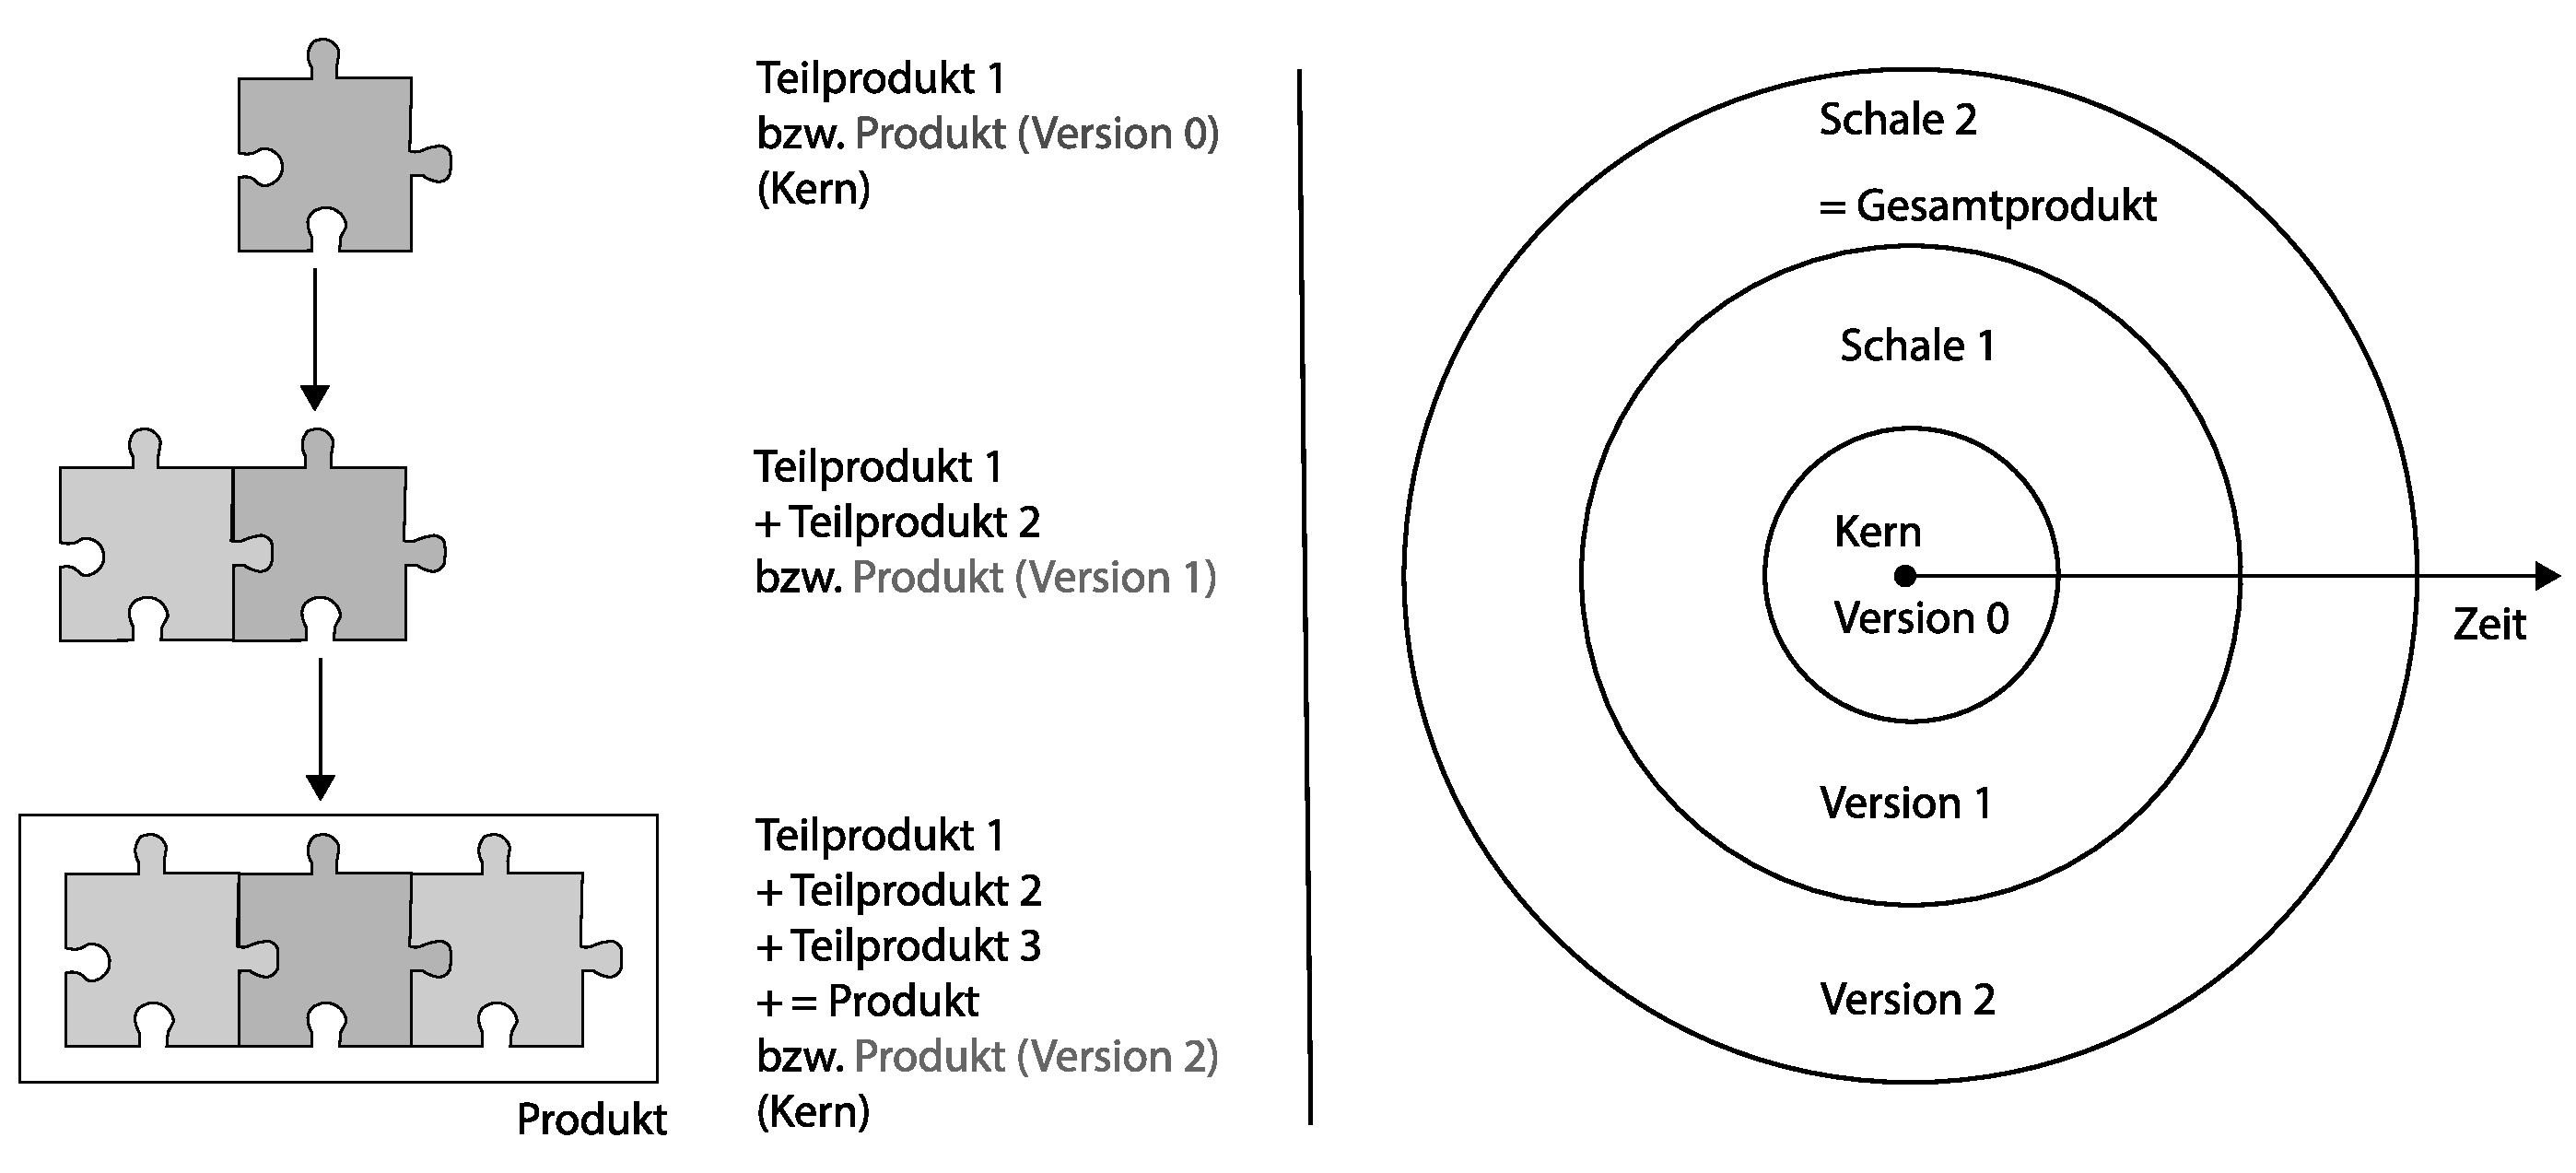
\includegraphics[width=1.2\textwidth]{Bilder/Kapitel-2/PuzzleZwiebel.pdf}
		\caption[Puzzleförmige und zwiebelschalenförmige inkrementelle Entwicklung]{Puzzleförmige (links) und zwiebelschalenförmige (rechts) inkrementelle Entwicklung, nach \cite[527]{bal08}}
		\label{fig:inkrementelle_entwicklung}
	\end{addmargin*}
	\end{addmargin*}
\end{figure}

Welche der beiden Arten 
\marginline{Entwicklungs\-prozess}
für ein konkretes Softwareentwicklungsprojekt eingesetzt werden sollte, hängt in erster Linie davon ab, in welcher Weise sich die Anforderungen an das Gesamtprodukt auf die geplanten Teilprodukte aufteilen lassen. Wenn sich die gewünschten Funktionalitäten annähernd eindeutig bestimmten Teilprodukten (\zb eine Passagierverwaltung und eine Flugzeugverwaltung für ein Flugreservierungssystem) zuordnen lassen, wird eher die puzzleartige Variante der inkrementellen Auslieferung zum Einsatz kommen. Bei der Planung der Inkremente müssen die zukünftigen Schnittstellen zwischen den Teilprodukten (in der Abbildung die Aus- und Einbuchtungen der Puzzleteile) dann so definiert werden, dass es im Ideal\-fall nicht nötig ist ein bestehendes Inkrement zu verändern, sobald ein weiteres Inkrement ergänzt wird.  Wenn dagegen geforderte Funktionalitäten unterschiedlicher Teilprodukte dieselbe Basis benötigen, ist es sinnvoll oder sogar zwingend notwendig, zunächst ein erstes Teilprodukt als Kern des Gesamtsystems zu entwickeln. Jedes weitere Inkrement baut dann so auf der vorherigen Pro\-dukt\-ver\-sion auf, dass es auf Basis der vorherigen Inkremente die Funktionalitäten des Produkts erweitert. Kombinationen beider Varianten der inkrementellen Auslieferung sind auch möglich, zum Beispiel falls alle Teilprodukte nur einen gemeinsamen Kern benötigen, ansonsten aber nicht aufeinander aufbauen müssen.

Die Entwicklung der Teilprodukte – auch bei puzzleförmiger Aufteilung – findet in der Regel nicht parallel, sondern zumindest versetzt statt (\zb Teilprodukt 1 schon im Einsatz, Teilprodukt 2 in der Entwicklung, Teilprodukt 3 in der Planung etc.). Dies dient auch dem Ziel, (positive und negative) Erfahrungen der Nutzer mit einer Produktversion bei der Erstellung der nächsten (erweiterten) Produktversion nach Möglichkeit berücksichtigen zu können. Eine grundlegende Überarbeitung schon ausgelieferter Teilprodukte sehen inkrementelle Modelle nicht vor; schon existierende Funktionalität wird – außerhalb von Fehlerbehebung und Schnittstellenanpassung – nicht verändert.

\sttpHervorhebung{\textbf{Inkrementelle Modelle}}
\marginline{Umgang mit Anforderungen}
\sttpHervorhebung{\textbf{erfordern eine klare Aufteilung der Anforderungen auf die Teilprodukte.}}
Zu Projektbeginn müssen die zentralen Anforderungen an das Gesamtprodukt soweit spezifiziert werden, dass eine Aufteilung in Teilprodukte und die Definition der Schnittstellen zwischen den Teilprodukten möglich sind. Detailliertere Entwurfs- und Implementierungstätigkeiten sind dann zunächst nur für das als erstes auszuliefernde Teilprodukt erforderlich. Der Einsatz inkrementeller Modelle erfordert die gewünschten Funktionalitäten des zukünftigen Softwareprodukts klar voneinander abzugrenzen, um sie den geplanten Inkrementen zuordnen und die Schnittstellen zwischen den Inkrementen definieren zu können. Dafür müssen insbesondere die Abhängigkeiten zwischen einzelnen Anforderungen noch detaillierter analysiert werden als bei Einsatz eines sequentiellen Vorgehensmodells. 

Abhängig vom konkreten inkrementellen Modell muss die (zukünftige) Anzahl der Inkremente zu Beginn des Softwareentwicklungsprojekts festgelegt werden, oder es können im Laufe des Projekts weitere (zukünftige) Inkremente definiert werden. Diese Frage ist eng verknüpft mit der Möglichkeit bzw. Unmöglichkeit im Laufe der Entwicklung neue Anforderungen zu berücksichtigen. Inkrementelle Modelle mit sequentiellem Charakter sehen vor, die vollständigen Anforderungen für alle zukünftigen Teilprodukte schon zu Projektbeginn zu erfassen, noch bevor mit Entwicklungstätigkeiten für das erste Teilprodukt begonnen wird. Andere inkrementelle Modelle sind diesbezüglich flexibler, haben dafür aber ein höheres Risiko, dass die zu Projektbeginn vorgesehene Architektur des Systems für die noch zu berücksichtigenden Anforderungen weniger gut oder im schlimmsten Fall gar nicht geeignet ist. In jedem Fall können neue oder veränderte Anforderungen an das Gesamtprodukt nur dann Berücksichtigung finden, wenn sie sich gut in noch zu entwickelnde Teil\-produkte integrieren lassen bzw. die Möglichkeit besteht zusätzliche Teilprodukte zu definieren. 

\sttpHervorhebung{\textbf{Inkrementelle Modelle}}
\marginline{Einbezug Kunde}
\sttpHervorhebung{\textbf{beziehen den Kunden stärker ein als sequen\-tiel\-le Modelle.}}
Inkrementelle Softwareentwicklung hat im Vergleich zu einem rein sequentiellen Vorgehen den Vorteil, dass der Kunde deutlich schneller eine erste einsetzbare Produktversion bekommt. Diese erste Produktversion kann zum Beispiel den Kern des zukünftigen Gesamtprodukts bilden, oder die für den Kunden wichtigsten Funktionalitäten beinhalten, oder die bezüglich des Entwicklungsaufwands am schwierigsten zu planenden Anforderungen umsetzen. In jedem Fall werden bei Einsatz von inkrementellen Modellen Missverständnisse oder Unklarheiten zwischen dem Entwicklungsteam und dem Kunden (\zb bezüglich der Anforderungen) früher sichtbar als bei sequentiellen Modellen. Das Risiko des kompletten Scheiterns des Softwareentwicklungsprojekts kann so verringert werden. Zudem können zwischen Auftraggeber und Auftragnehmer anstelle eines einzigen Vertrags über die Entwicklung des Gesamtprodukts auch (zeitversetzt abgeschlossene) Verträge für einzelne Teilprodukte vereinbart werden.

Inwieweit der Kunde in den konkreten Entwicklungsprozess der Teilprodukte einbezogen wird, hängt vom konkret eingesetzten inkrementellen Modell ab. Folgt es eher sequentiellen Ansätzen, wird der Kunde nur für Prozesse der Anforderungsermittlung und für die Abnahme der einzelnen Teilprodukte einbezogen. Inkrementelle Modelle, die auch Methoden aus dem agilen Umfeld einsetzen, beinhalten dagegen in der Regel institutionalisiertes und durchgehendes Feedback des Kunden über den gesamten Zeitraum der Entwicklung.

Wie in Abschnitt~\ref{sec:Kap-2.2.1} erwähnt, 
\marginline{Artefakte} 
sind \textbf{sequentielle} Modelle in der Regel dokumentenorientiert. Bezüglich der inkrementellen Modelle finden sich in der Literatur in dieser Hinsicht unterschiedliche Darstellungen. Dies ist wieder der großen Spannweite inkrementeller Modelle geschuldet. Inkrementelle Modelle, die sequentielle \mbox{Methoden} einsetzen, werden eher dokumentenorientiert sein; inkrementelle Modelle mit iterativen oder agilen Methoden eher code- oder testorientiert.


\minisec{Iterative Modelle}

Im Unterschied zu (klassisch) inkrementellen Modellen ist es essentieller Bestandteil von \textit{iterativen Modellen}, dass auch lauffähige (und auch schon ausgelieferte) Produktversionen verändert werden; zum Beispiel weil sich Anforderungen geändert haben bzw. zuvor noch nicht detailliert erfasst waren, neue Anforderungen hinzugekommen sind, Entwurfsentscheidungen revidiert werden, auf neuere Technologien gesetzt werden soll etc. 

Wie bei den inkrementellen Modellen ist die Spannweite an Modellen, die man als iterative Modelle bezeichnen könnte, groß. Am einen Ende stehen sequentielle oder inkrementelle Modelle, wenn sie in größerem Umfang auch iterative Methoden einsetzen. Am anderen Ende stehen die agilen Modelle, die gleichzeitig iterative Modelle sind.

Ziel von iterativen Modellen ist die Verbesserung des Softwareprodukts mit jeder Überarbeitung. Verbessern kann heißen, dass neue Funktionalität hinzugefügt wird, aber auch, dass Aspekte wie die Bedienbarkeit der Software, die Wiederverwendbarkeit einzelner Komponenten, die Schnittstellen zu anderen Systemen oder auch die interne Datenstruktur überarbeitet werden. Dabei ist es möglich, Arbeiten aus vorherigen Iterationen wieder zu verwerfen. Die Dauer einer Iteration hängt stark vom konkreten Softwareentwicklungsprojekt ab. In der Regel liegt sie zwischen einigen Wochen und wenigen Monaten und ist damit deutlich geringer als die Entwicklungszeit eines Inkrements – sprich eines kompletten Teilprodukts – in klassisch inkrementellen Modellen.

\sttpHervorhebung{\textbf{Iterative Modelle}} 
\marginline{Entwicklungs\-prozess}
\sttpHervorhebung{\textbf{durchlaufen die Kernprozesse des Softwareengineering in Zyklen.}} 
In iterativen Vorgehensmodellen wird zunächst anhand einiger Basis\-anforderungen eine erste Kernversion, teilweise auch Nullversion genannt, entwickelt. Kennzeichnend (und namensgebend) für die iterativen Modelle ist, dass die Prozesse des Softwareengineering ausgehend von dieser Kernversion im weiteren Verlauf der Produktentwicklung wiederholt durchlaufen werden und mit jedem Zyklus (jeder Iteration) eine neue, erweiterte oder angepasste Produktversion entsteht, die die vorherige ablöst. Das erinnert auf den ersten Blick an die oben dargestellte zwiebelschalenförmige inkrementelle Entwicklung. Im Gegensatz zu dieser ist die (unter Umständen auch weitreichende) Überarbeitung der aktuellen Version aber ein zentrales Kennzeichen iterativer Modelle. Im Unterschied zu sequentiellen Modellen sind die einzelnen Softwareengineering-Prozesse in iterativen Modellen zudem in der Regel deutlich schwächer voneinander abgegrenzt. So können zum Beispiel Entwurfs- und Implementierungstätigkeiten oder Implementierungs- und Testtätigkeiten eine Einheit bilden und Hand in Hand stattfinden. Und selbst wenn die einzelnen Prozesse innerhalb einer Iteration nacheinander ausgeführt werden, werden sie nicht wie in sequentiellen Modellen durch formale Meilensteine voneinander getrennt. 

\begin{figure}[h!]
	\centering
	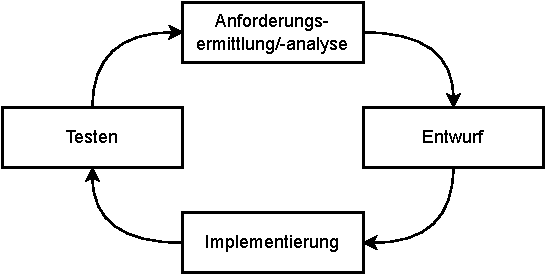
\includegraphics[scale=1.0]{Bilder/Kapitel-2/Abb-2-9.pdf}
	\caption[Iterative Softwareentwicklung]{Iterative Softwareentwicklung. Eine Iteration entspricht einem Zyklus in der Abbildung. Die mögliche zwischenzeitige Auslieferung von lauffähigen Versionen ist hier in der Abbildung nicht berücksichtigt.}
	\label{fig:iterative_softwareentwicklung}
\end{figure}

Durch die Entwicklung des Produkts als Folge von Iterationen kann das Entwicklungsteam von den gesammelten Erfahrungen während einer Iteration profitieren und damit nicht nur das Produkt, sondern auch die Arbeitsprozesse in den folgenden Iterationen optimieren. Im Unterschied zu sequentiellen Modellen, bei \mbox{denen} die verschiedenen Phasen (\zb Entwurf, Implementierung) sehr unter\-schied\-liche Arbeitsprozesse verlangen, sind sich die einzelnen Entwicklungsabschnitte eines iterativen Modells deutlich ähnlicher: die Prozesse des Softwareengineering werden in jeder Iteration erneut durchlaufen – wenn auch in einigen Vorgehensmodellen mit unterschiedlicher Schwerpunktsetzung. Somit können als ungünstig empfundene Arbeitsprozesse einer Iteration direkt in der nächsten Iteration verbessert werden. Ähnliches gilt übrigens auch für die eingesetzten Softwareentwicklungswerkzeuge  (\zb Entwicklungsumgebungen, Modellierungstools, Test-Frameworks). %\sttpgls{CASE_Tools}
Diese können in folgenden Iterationen gewechselt werden, wenn andere Werkzeuge geeigneter erscheinen. In sequentiellen Modellen können positive und negative Erfahrungen mit durchgeführten Arbeitsprozessen oder eingesetzten Werkzeugen dagegen erst im nächsten Softwareentwicklungsprojekt berücksichtigt werden.

\sttpHervorhebung{\textbf{In iterativen Modellen}}
\marginline{Einbezug Kunde}
\sttpHervorhebung{\textbf{wird der Kunde frühzeitig einbezogen.}}
Die Entwicklung in Iterationen erleichtert es, den Kunden in den Entwicklungsprozess einzubinden, zum Beispiel indem nach Abschluss jeder Iteration Rückmeldungen des Kunden eingeholt werden. Dabei besteht die Möglichkeit, anhand der aktuellen Version bzw. des aktuellen Stands Anforderungen für die nächste Version bzw. den nächsten Entwicklungsabschnitt zu verfeinern oder sogar neue Anforderungen zu spezifizieren. Gerade nicht technisch versierten Kunden fällt es sehr viel leichter, auf Grundlage schon funktionierender Software bzw. Prototypen Anforderungen oder Änderungswünsche zu äußern.
%\sttpgls{Prototyp} 

Um  Rückmeldung vom Kunden zu erhalten, kann die aktuelle Produktversion produktiv eingesetzt werden, der Kunde seine Erfahrungen sammeln und für die nächste Version kommunizieren. Rückmeldung kann aber auch heißen, dass die Version nur im Rahmen einer Produktvorstellung vom Kunden kommentiert wird und nicht produktiv eingesetzt wird. Bei letzterer Variante kann es sich dann um lauffähigen Code handeln – die Version somit potentiell produktiv einsetzbar sein – muss es aber nicht (\zb nur animierte Benutzungsschnittstellen). Für produktiv eingesetzte Versionen wird in der Literatur manchmal der Begriff \textit{Release}
\marginline{Release}
verwendet, der auch im Umfeld agiler Modelle verbreitet ist.

\pagebreak %%% für Druck

\sttpHervorhebung{\textbf{Iterative Modelle berücksichtigen Anforderungsänderungen.}} \marginline{Umgang mit Anforderungen}
Iterative Vorgehensmodelle können durch die kürzeren Entwicklungszyklen und die stärkere Einbindung des Kunden besser als inkrementelle Modelle und deutlich besser als sequentielle Modelle mit zusätzlichen oder veränderten Anforderungen während der Projektlaufzeit umgehen. Zudem tragen sie explizit der Tatsache Rechnung, dass es auch bei zu Projektbeginn feststehenden und stabilen Anforderungen aufgrund von Missverständnissen zwischen Kunden und Entwicklungsteam vorkommen kann, dass die Umsetzung nicht den (eigentlichen) Wünschen des Kunden entspricht. 

Iterative  Modelle sind daher gut geeignet, wenn die Funktionalitäten des zukünftigen Produkts zu Beginn der Entwicklung noch nicht komplett feststehen oder auf Änderungen während der Entwicklung reagiert werden soll. Letzteres bezieht sich im Übrigen nicht nur auf Änderungen der Anforderungen, sondern auch auf technologische Änderungen (\zb Verfügbarkeit passenderer Frameworks). Auf der anderen Seite besteht bei iterativen Modellen immer die Gefahr, dass die für die Kernversion gewählte Systemarchitektur sich in späteren Iterationen als zu unflexibel für den Einbau weiterer Funktionalität herausstellt und (aufwändig) überarbeitet werden muss. Diese Gefahr ist umso größer, je weniger klar der Kunde die Funktionalitäten des zukünftigen Softwareprodukts zu Projektbeginn spezifizieren kann. Wenn die fachlichen oder technologischen Unsicherheiten des Produkts zu Projektbeginn sehr groß sind, kann es sinnvoll sein iterative Modelle zusätzlich mit Verfahren aus dem Prototyping 
%\sttpkapitelverweis{Pro\-to\-typen\-ent\-wick\-lung}{Kap.~\ref{sec:Kap-7}}
zu verbinden. 

Aus Managementsicht liegt eine Schwierigkeit von iterativen Modellen in der Kontrolle des Projektfortschritts. Wenn zu Beginn des Entwicklungsprojekts nicht komplett feststeht, über welche Funktionalitäten das zu entwickelnde Produkt bei Fertigstellung verfügen wird, ist es während der Projektlaufzeit schwierig bis unmöglich zu beurteilen, ob der Entwicklungsfortschritt zu einem bestimmten Zeitpunkt im Zeitrahmen liegt oder nicht. Ebenfalls aufgrund der nicht vollständigen Spezifizierung der Anforderungen zu Projektbeginn ist auch die Vertragsgestaltung kompliziert, wenn ein Softwareprodukt nicht für das eigene Unternehmen, sondern für einen Auftraggeber entwickelt werden soll. Dieses Problem wurde in den 2000er Jahren mit dem stärkeren Einsatz agiler Vorgehensmodelle, bei denen die iterative Entwicklung essentieller Bestandteil ist, weithin sichtbar. Lösungsmöglichkeiten sind vorgeschaltete Prototyping-Projekte und neue Arten von Vertragsmodellen.

\sttpHervorhebung{\textbf{Iterative Modelle sind code- oder testorientiert.}} \marginline{Artefakte}
Codeorientiert bedeutet, dass am Abschluss jeder Iteration Programmcode steht. Iterative Modelle können (darüber hinaus) auch testorientiert sein, wenn Iterationen eine Menge zuvor spezifizierter Testfälle zugrunde liegen, die die jeweilige Produktversion der Software erfüllen soll. Basis für solche Testfälle können zum Beispiel typische Arbeitsabläufe sein, die die zukünftige Software unterstützen soll. 
%\sttpkapitelverweis{Use Cases}{Kap.~\ref{sec:Kap-6.2.1.1}}
%\sttpkapitelverweis{User Stories}{Kap.~\ref{sec:Kap-6.2.1.2}}

Anders als bei sequentiellen Modellen entstehen bei iterativen Modellen aufgrund der Verschmelzung der Softwareengineering-Prozesse und der starken Codeorientierung nicht automatisch während des Entwicklungsprozesses (Meilenstein)-Dokumente, wie eine strukturierte Auflistung der Anforderungen, eine Übersicht über alle Komponenten der Software, eine detaillierte Beschreibung einzelner Funktionen oder auch eine Historie getroffener Entwurfsentscheidungen etc. Eine Schwierigkeit iterativer Modelle besteht daher darin, wie das zukünftige Produkt und getroffene Entscheidungen dokumentiert werden. Eine entsprechende Dokumentation müsste parallel zur Implementierung innerhalb einer Iteration erstellt und bei Änderungen in späteren Iterationen immer wieder angepasst werden. Es ist stark abhängig vom konkreten Softwareentwicklungsprojekt, wie weitreichend eine Dokumentation des Systems und der getroffenen Entscheidungen in iterativen Modellen vorgenommen wird. Die minimale Variante ist der weitgehende Verzicht einer externen Dokumentation, indem der Programmcode möglichst „selbsterklärend“ gestaltet wird und nur um absolut notwendige Kommentare sowie um Funktionalitätsbeschreibungen von Schnitt\-stellen ergänzt wird. Weitergehendere Varianten wären die zusätzliche externe (und in späteren Iterationen jeweils anzupassende) Dokumentation der Anforderungen zum Beispiel anhand von User Stories oder die Dokumentation der Systemstruktur zum Beispiel anhand von Komponenten- und Klassendiagrammen. %\sttpkapitelverweis{Komponenten\-diagramme}{Kap.~\ref{sec:Kap-6.1.2}}
%\sttpkapitelverweis{Klassendiagramme}{Kap.~\ref{sec:Kap-3.2.4}} 
Weitreichende externe Dokumentationen dokumentieren darüber hinaus auch getroffene Entscheidungen und ihre Gründe – sei es klassisch in Form von Dokumenten oder agiler über Wikis oder Ticketsysteme –, um validere Folgeabschätzungen zu ermöglichen, falls getroffene Entscheidungen im späteren Projektverlauf revidiert werden müssen.

Das erste Vorgehensmodell, das umfangreichere Iterationen vorsah, war Ende der 1980er Jahre das Spiralmodell von Barry W. Boehm (\cite{boe86} und \cite{boe88}). Aus heutiger Sicht liegt die Bedeutung des Spiralmodells vor allem darin, dass es schon in den 1980er Jahren – und damit zur Hochzeit der phasenorientierten Modelle – ein iteratives Vorgehen und den Einsatz von Prototypen für die Entwicklung eines Softwareprodukts propagierte. Deutlich bekannter geworden ist aber der  im Zuge der objektorientierten Programmierung in den 1990er Jahren groß gewordene (Rational) Unified Process.

\sttpAutorenkasten{Barry W. Boehm}{1935}{2022}{
	\vspace{2mm} %%% für Druck
	US-amerikanischer Software\-ingenieur. Neben seiner Arbeit an Vorgehensmodellen ist er vor allem für das COCOMO-Modell bekannt. COCOMO (Constructive Cost Model) ist ein algorithmisches Modell, mit dem Kosten und Aufwand von geplanten Softwareprojekten geschätzt werden können.
	\vspace{2mm} %%% für Druck
}{Bilder/Autoren/boehm.jpg}{2006}{Improve it, \href{https://creativecommons.org/licenses/by-sa/2.0}{CC BY-SA 2.0}, via \href{https://commons.wikimedia.org/wiki/File:O_lend\%C3\%A1rio_Barry_Boehm.jpg}{Wikimedia Commons}}

